\documentclass[17pt, a1paper, portrait]{tikzposter}
\usepackage[utf8]{inputenc}
\usepackage{graphicx}
\usepackage{amsmath}
\graphicspath{{./poster\_images/}}
\usepackage{xcolor}
\usepackage{changepage}
\definecolor{eurecomblue}{RGB}{0,159,227}
\definecolor{visuwalkorange}{RGB}{255,204,0}



% RAJOUTER TITRE DU PROJET, AUTEURS
% 30% TEXTE, 40% ILLU, 30% VIDE
% PRECISER CHALLENGE TECHNIQUES
% RESULTATS
% CONCLUSION
% AMELIORATIONS, REFERENCES



\definebackgroundstyle{eurecom}{
\node[inner sep=0pt] at (0,0){
    
\includegraphics[width = \paperwidth,
    height = \paperheight]
    {poster-template.pdf}};
}

\defineblockstyle{bestblockstyle}{
titlewidthscale=0.9, bodywidthscale=1,titleleft,
titleoffsetx=0pt, titleoffsety=0pt, bodyoffsetx=0mm,
bodyverticalshift=10mm, roundedcorners=5,
titleinnersep=5mm, bodyinnersep=4mm,
bodyoffsety=8mm
}
{
\draw[color=eurecomblue, fill=blockbodybgcolor, line width=3pt,
rounded corners=\blockroundedcorners] (blockbody.south west)
rectangle (blockbody.north east);
\ifBlockHasTitle
\draw[color=eurecomblue, fill=eurecomblue
, line width=2pt
rounded corners=\blockroundedcorners] (blocktitle.south west)
rectangle (blocktitle.north east);
\fi
}

%TODO: maybe, remove watermark (bottom right of the page)

\usetitlestyle{Empty}

\usebackgroundstyle{eurecom}
\title {\hspace{-40cm}Visuwalk}

\titlegraphic{\hspace{-40cm}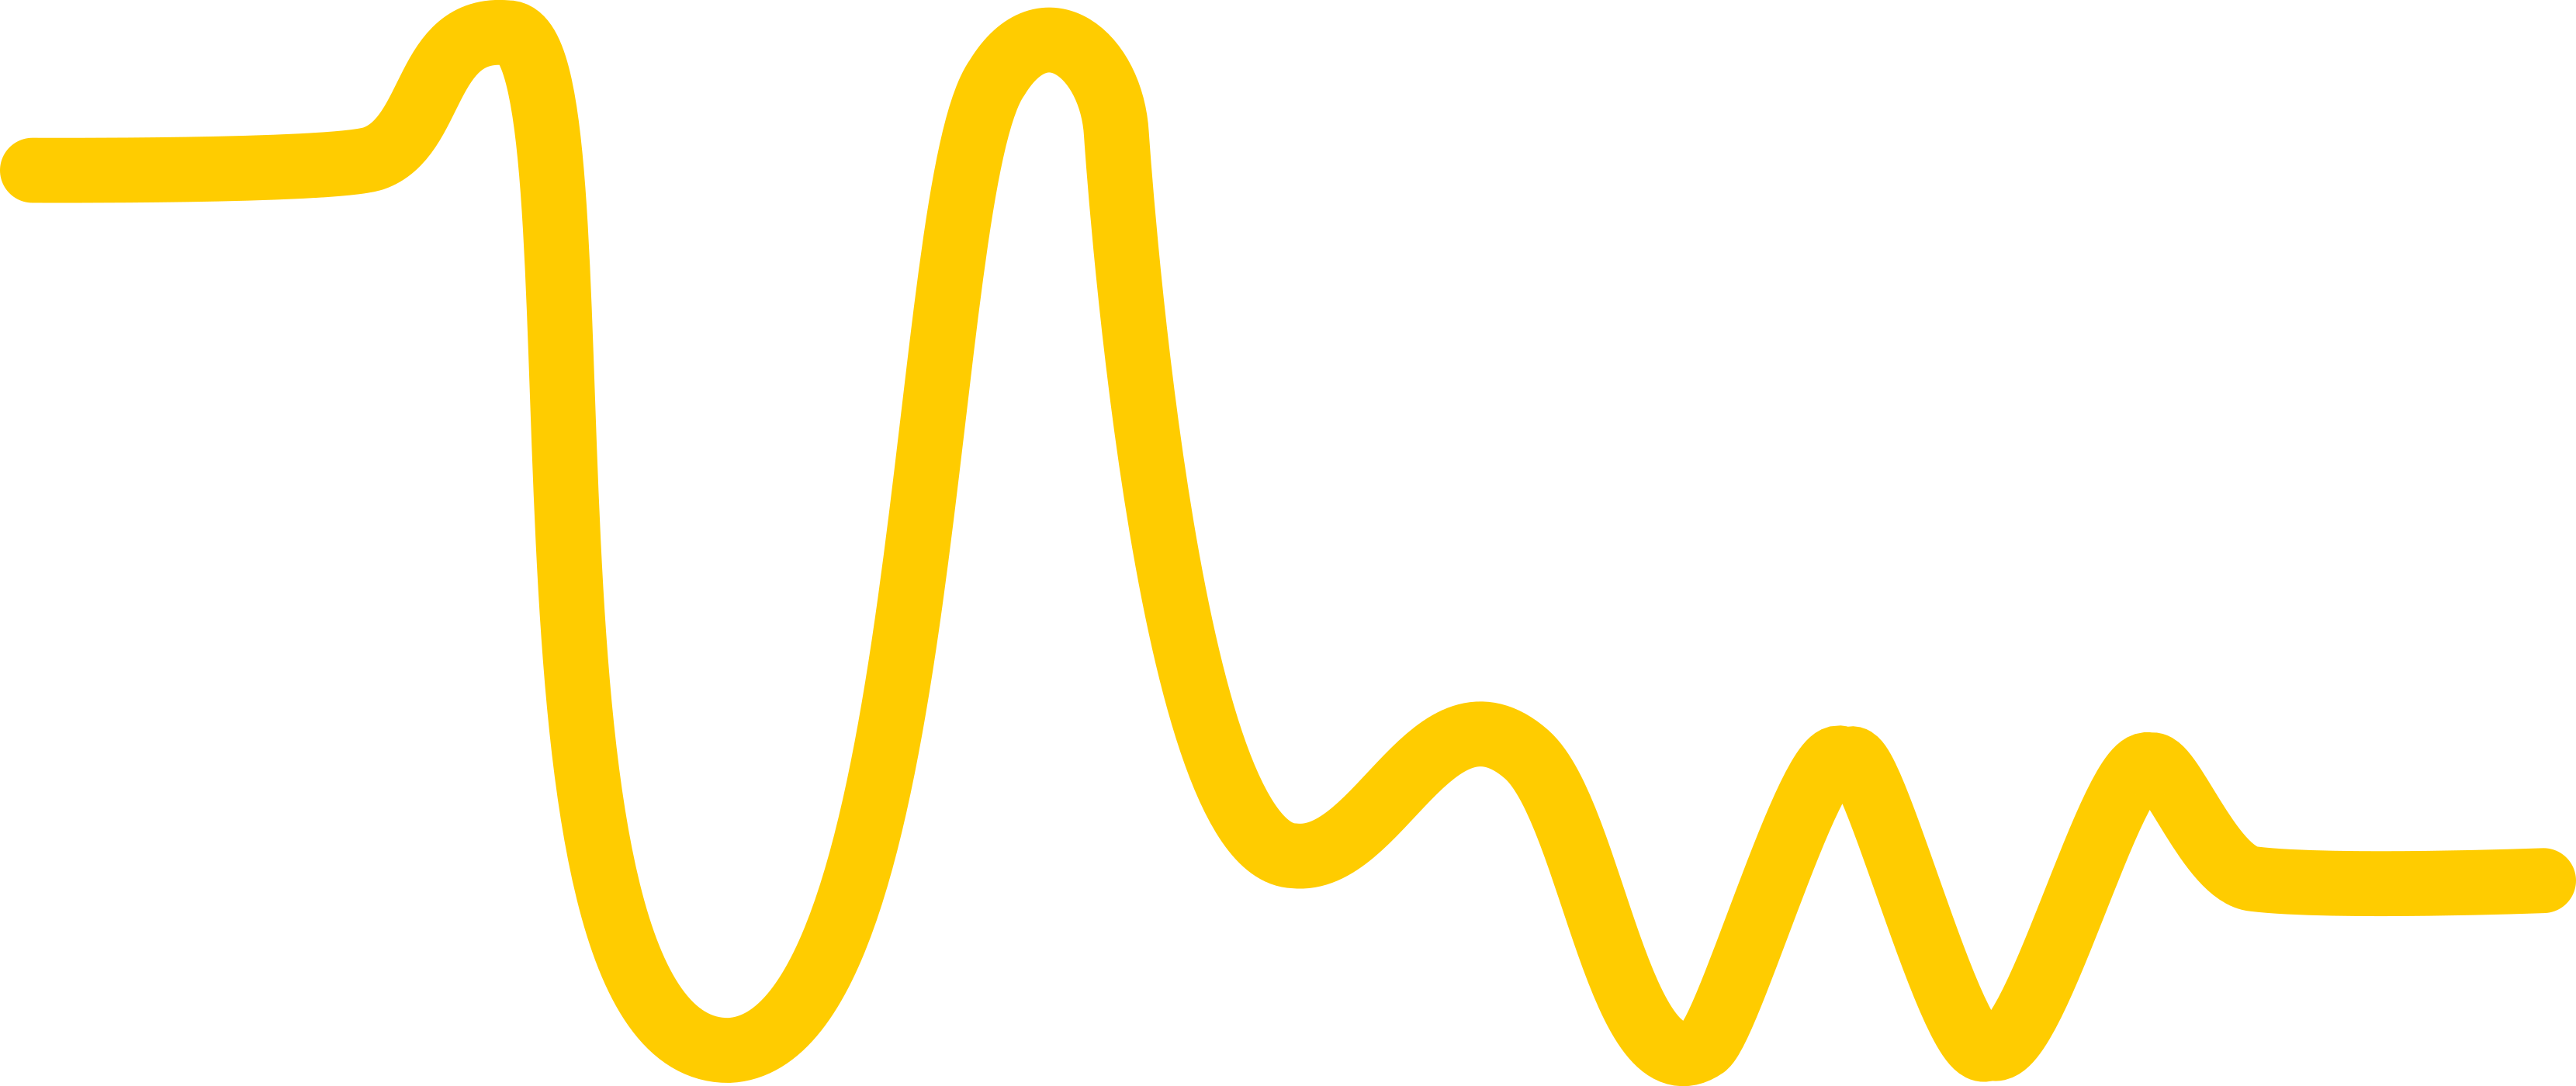
\includegraphics[width=0.20\paperwidth]{logo1.png}}
\author{\hspace{-40cm}\large Alexandre Avy, Hichem Khettab, Lou Marze, \\ \hspace{-40cm} Hamza Parnica, Guillaume Ung}
\date{Semester 5}

\begin{document}


\useblockstyle{bestblockstyle}

\maketitle[titletotopverticalspace=90mm,width = 0.5\paperwidth]

\block[titleoffsety=13cm,bodyoffsety=138mm,bodyverticalshift=10mm,titleinnersep=5mm,bodyinnersep=4mm,bodyoffsetx=80mm,bodywidthscale=.72,titlewidthscale=.4]{\textbf {Abstract}}{
\Large
% TODO: add phrase d'accroche on blind people et les besoins et la raison pour ce projet etc.
The goal of this semester project is to guide ,with sounds, a visually impaired person to follow a line. \\
The available tools are a Rasperry Pi and its camera.
For this goal, one needs to : \\
Detect the line from the camera's video \\
Process the line with the right technique \\
Find a way to communicate instructions to the user
}

\begin{columns}

\column{0.5}

\block{
\textbf{Video Processing}}{

\begin{center} \LARGE {Detecting the line}
\end{center}

\vspace{2mm}

\begin{center}
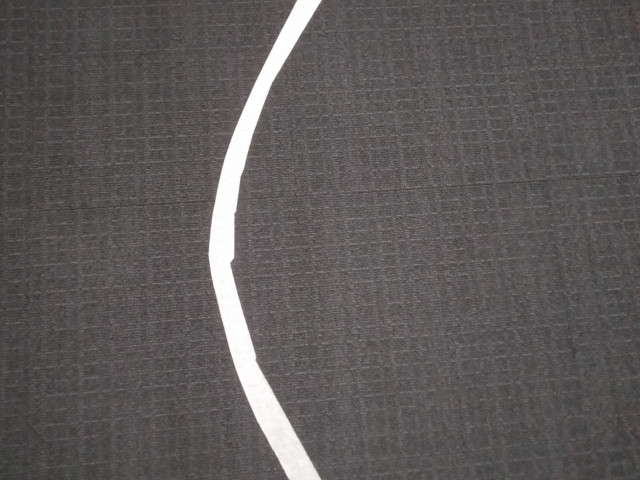
\includegraphics[height = 6cm, width = 6cm]{poster_images/reel3.jpg}
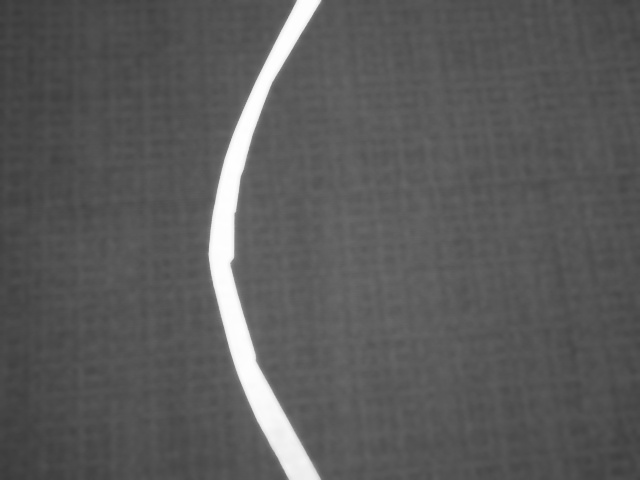
\includegraphics[height = 6cm, width = 6cm]{poster_images/gray.jpg}
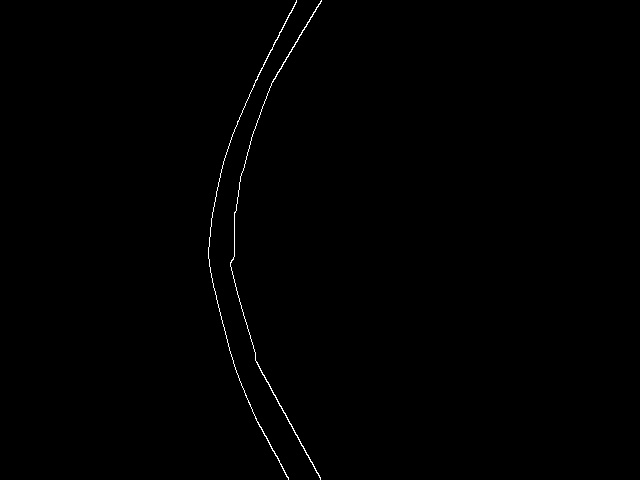
\includegraphics[height = 6cm, width = 6cm]{poster_images/canny_edge.jpg}
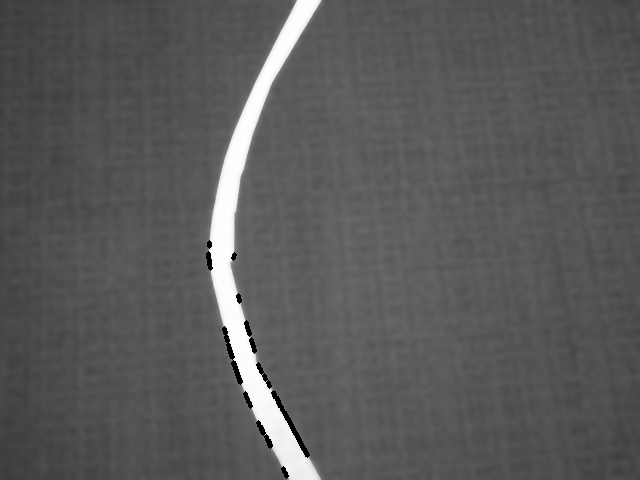
\includegraphics[height = 6cm, width = 6cm]{poster_images/houghlines_maybe.jpg}
\caption{\emph{Original image/Filtered image/Canny edge detection/Lines from Hough transform}}
% \centering\large Original image / Bilateral filter / Canny edge detection / Lines from Hough transform
\end{center}

Prior to detecting the line, the image is processed to optimize the detection quality through: \\
- Bilateral filtering \\
- Canny edge detection \\
Then Hough transform is applied to detect straight lines in the edges image.
 

% TODO: add caption, resize image and spacing
\vspace{2mm}

\begin{center} \LARGE {Computing the line direction}
\end{center}

\begin{center}
\frame{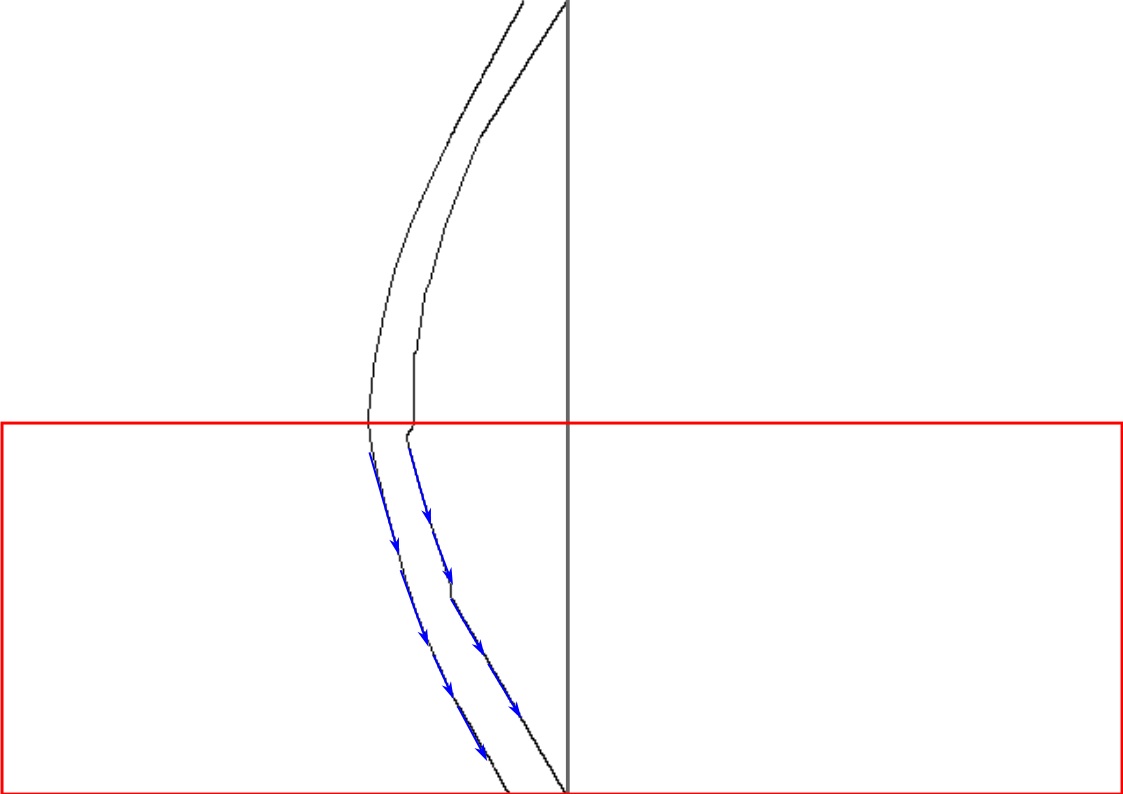
\includegraphics[width=0.45\linewidth,height = 8cm]{poster_images/angle_alpha1.png}}
\frame{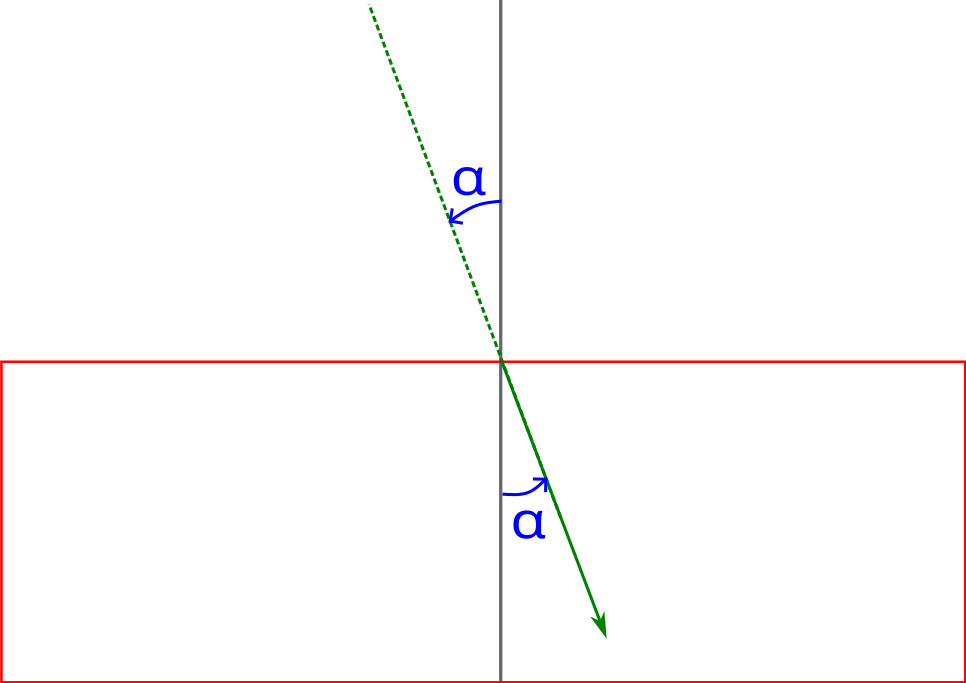
\includegraphics[width=0.45\linewidth,height = 8cm]{poster_images/angle_alpha.png}}
\centering
\caption{\emph{Detected lines on bottom of the frame / Representation of the \(\alpha\) angle}}
\end{center}
The \(\alpha\) angle is defined as the average angle of the detected lines. We take only the bottom of the image into account, in order not to communicate a direction too early to the user and get
out of the line.

% TODO: add caption, resize image and spacing

\begin{center} \LARGE {Taking the user position into account}
\end{center}


% \begin{center}
% \hspace{-0.7\linewidth}
% \includegraphics[width=0.2\linewidth]{poster_images/distance_bas_barycentre.png}
% \end{center}

% \begin{center}
% \hspace{0.2\linewidth}
% \vspace{90mm} \large dbneufnuizbnfueabfieja
% \end{center}
}

\column{0.5}

\block{}{

Along with giving the line direction, it should also be taken into account that
the user could deviate from the line and needs to get back to it quickly. \\
For this purpose, we take a look at the distance \(d\) of the barycentre of the
pixels detected as edges, at the bottom of the line, with the middle of the
image (considered as the user's position).

\begin{center}
\includegraphics[width=0.2\linewidth]{distance_bas_barycentre.png}
\end{center}

Then, if the distance is too important, the user should be given the
information to get back on the line instead of following its curve, because he
is no longer on it. \\
In order to do this, we define the \(\beta\) angle as the angle between the
barycentre of a fine-tuned target zone (towards the user should go) and the
user itself. This target zone is not perpendicular to the user but is choosen a
little more ahead, so that the changes in direction are not enormous and that
the time spent to get back to the line is not huge too (reminding that it is a
race).

\begin{center}
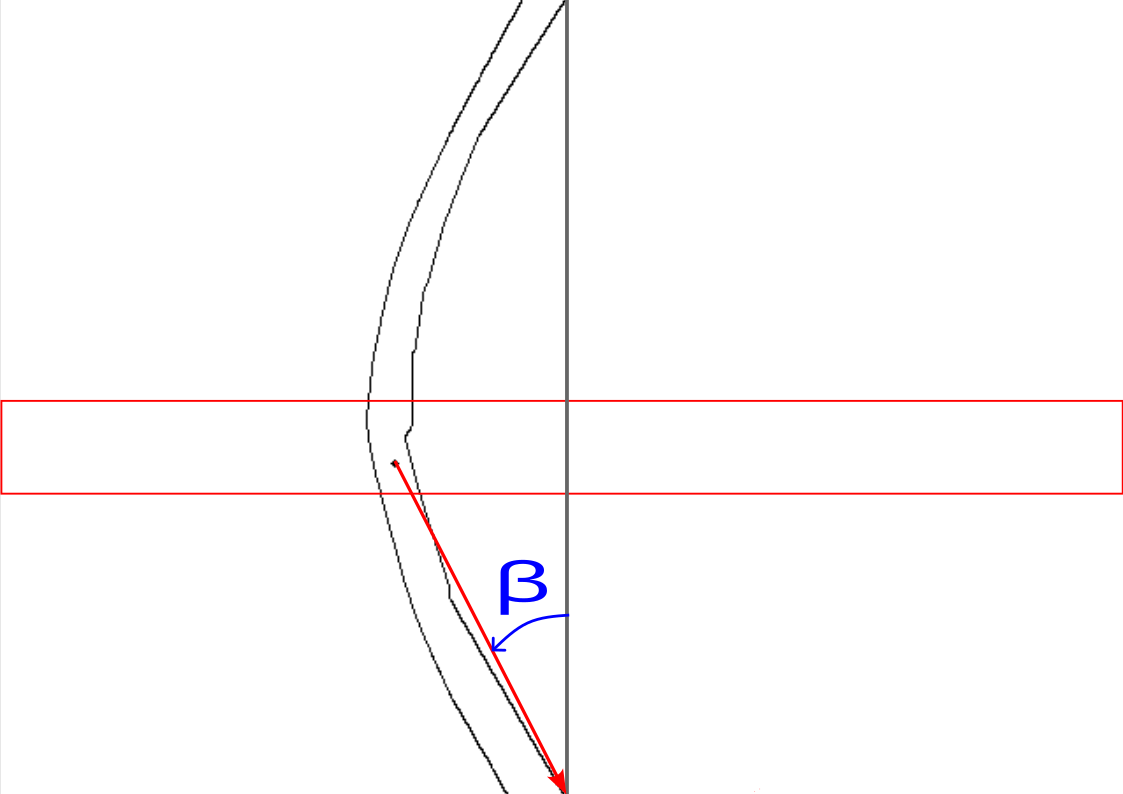
\includegraphics[height = 7cm, width = 6cm]{poster_images/angle_beta_barycentre_targetpoint.png}

\large l'angle beta wow
\end{center}

}

\block{Information processing}{
We want the final angle to reflect the distance of the user to the line, i.e.
we take more \(\alpha\) into account when \(d\) is small than \(\beta\), and
vice-versa. \\
Thus, we need a function \(f(d)\) that is close to 0 when \(d\) is small, and
close to 1 when \(d\) is big.

%TODO: add tikz figure de f(d) seulement

We choose

\[ f(d) = (1 - e^{\frac{-d}{\tau}}) \]

We choose \(\tau\) so that \(d_{95\%} = \frac{\text{width}}{2}\), thus we
have
\[ 3\tau = \frac{\text{width}}{2}, \quad \tau = \frac{\text{width}}{6} \]
It follows,
\[f(d) = 1 - e^{\frac{-6d}{\text{width}}}\]

Finally, we have

\[ \gamma = e^{\frac{-6d}{\text{width}}}\alpha + (1 - e^{\frac{-6d}{\text{width}}})\beta \]
\[ \gamma = \alpha + (1 - e^{\frac{-6d}{\text{width}}})(\beta - \alpha) \]

% TODO: ajouter tikz plot des deux termes et de gamma(d)
}

\block{\textbf{Sound Processing}}{}

\end{columns}
\block{\textbf{Conclusion}}{}
\end{document}
    